
\lecture{Hypothesis Testing}{hypothesis-testing}
\section{Hypothesis Testing}

\title{Hypothesis Testing Where the Standard Deviation is Known}
\subtitle{Is there a difference?}

%\author{Kelly Black}
%\institute{Clarkson University}
\date{6 November 2013}

\begin{frame}
  \titlepage
\end{frame}

\begin{frame}
  \frametitle{Outline}
  \tableofcontents[hideothersubsections,sectionstyle=show/hide]
\end{frame}



\subsection{Clicker Quiz}



\begin{frame}
  \frametitle{Clicker Quiz}

  % \begin{clickerQuiz}

  \iftoggle{clicker}{%
    
    Cereal is produced at one of your factories. You are told that the
    mean contents is 417.3g per box. You suspect that this is too
    high. 

    What hypothesis test would you form to test this? \\
    ~ \\
    \begin{tabular}{ll@{\hspace{3em}}l}
      A & $H_0$: The mean is less that 417.3g  \\
        & $H_a$: The mean is  417.3g \\
      ~ \\
      B & $H_0$: The mean is 417.3g \\
        & $H_a$: The mean is more than 417.3g \\
      ~ \\
      C & $H_0$: The mean is 417.3kg  \\
        & $H_a$: The mean is less than 417.3kg 
    \end{tabular}

  }

  %\end{clickerQuiz}
  

\end{frame}


\subsection{Hypothesis Testing}

\begin{frame}{Problem}

  \vfill

  $\bar{x}$ is a random variable.

  \vfill

  The data can \textbf{lie}!

  \vfill
  
\end{frame}


\begin{frame}{The Possibilities}

  \centerline{
\includegraphics[width=6.0cm]{img/hindenburg}}

  \begin{eqnarray*}
    \mathrm{Data~-} & &
      \begin{array}{l@{\hspace{1em}}|c|c|} 
        \multicolumn{3}{r}{\mathrm{Reality}} \\ 
        \multicolumn{1}{c}{~} & \multicolumn{1}{c}{H_0
          \mathrm{~is~true}} & \multicolumn{1}{c}{H_0
          \mathrm{~is~false}} \\  
        \hhline{~--}
        \mathrm{Do~Not~Reject~}H_0 & 
\includegraphics[width=0.7cm]{img/smiley} & \mathrm{Type~II~Error} \\ \hhline{~|-|-|}
        \mathrm{Reject~}H_0 & \mathrm{Type~I~Error} & 
\includegraphics[width=0.7cm]{img/smiley} \\ \hhline{~--}
      \end{array}
  \end{eqnarray*}
  
\end{frame}


\begin{frame}{How To State Results}

  How you state your conclusions matter! It is an ethical issue in
  terms of conveying your assumptions and potential problems
  associated with the methodology.

  \begin{block}{Reject $H_0$}
    There is sufficient evidence to reject $H_0$ at the \#
    significance level assuming a $t$-distribution with \# degrees of
    freedom and a standard deviation of \#.
  \end{block}

  \begin{block}{Cannot Reject $H_0$}
    There is not sufficient evidence to reject $H_0$ at the \#
    significance level assuming a $t$-distribution with \# degrees of
    freedom and a standard deviation of \#.
  \end{block}

  
\end{frame}

\begin{frame}{The Methodology}

  What do we do?

  \begin{enumerate}
  \item Assume that $H_0$ is true.
  \item Ask, ``Are the data an unlikely result?''
  \end{enumerate}

  \only<2->
  {
    We want:
    \begin{itemize}
    \item The probability that we get our result to be ``small.''
    \item The probability that we get our result \textit{given our
        assumptions} is the significance level
      ($\alpha$). \textbf{\color{red} It is a conditional
        probability!}
    \end{itemize}
  }

  \only<3->
  {
    Note: We need to define this cut-off value, $\alpha$, \textbf{in
      advance!} i.e. before any data collection or manipulation.
  }
  
\end{frame}


\subsection{Examples}

\begin{frame}{Example}

  A new type of fertilizer is trialed. Previous results indicated a
  mean height of the corn at harvest to be 2.80m. A sample of fourteen
  plants with the new fertilizer gave a sample mean of 2.93m and a
  sample standard deviation of 0.20m. Does the new fertilizer give a
  higher mean height?

  \vfill

  \only<2->
  {
    \begin{tabular}{l@{\hspace{2em}}l}
      $H_0$: & $\mu = 2.80$m \\
      $H_a$: & $\mu > 2.80$m
    \end{tabular}
    \\ Use a 5\% significance level. (Need to decide this first!)
  }

  \vfill

  \only<3->
  {
    We cannot reject the null hypothesis at the 95\% confidence level
    assuming a $t$-distribution with thirteen degrees of freedom.
  }

  \vfill

\end{frame}



\begin{frame}{Notation}

  $H_0:\mu=8$ vs. $H_a:\mu\neq 8$, $z^{*}=1.95$.

  \vfill

  $H_0:\mu=8$ vs. $H_a:\mu > 8$, $z^{*}=1.85$.

  
\end{frame}



\iftoggle{clicker}{%
  \begin{frame}
    \frametitle{Clicker Quiz}

    \vspace*{-1.5em}
    Fertilizer is produced and the amount of nitrogen is estimated to
    be 0.300 kg per cubic meter. A new process is put in place and
    tested. After eighteen trials a sample mean of 0.287 kg per cubic
    meter and a standard deviation of 0.030 kg per cubic meter is
    found. Does the new method make a difference?

    What hypothesis test would you form to test this? \\
    ~ \\
    \begin{tabular}{ll@{\hspace{3em}}l}
      A & $H_0$: The mean is 0.300 kg per cubic meters. \\
        & $H_a$: The mean is less than 0.300 kg per cubic meters. \\
        ~ \\
      B & $H_0$: The mean is 0.300 kg per cubic meters. \\
        & $H_a$: The mean is more than 0.300 kg per cubic meters. \\
        ~ \\
      C & $H_0$: The mean is 0.300 kg per cubic meters. \\
        & $H_a$: The mean is not 0.300 kg per cubic meters. \\
        ~ \\
      D & $H_0$: The mean is not 0.300 kg per cubic meters. \\
        & $H_a$: The mean is 0.300 kg per cubic meters. \\

      \end{tabular}

    \end{frame}
}


\begin{frame}{Example}

    Fertilizer is produced and the amount of nitrogen is estimated to
    be 0.300 kg per cubic meter. A new process is put in place and
    tested. After eighteen trials a sample mean of 0.287 kg per cubic
    meter and a standard deviation of 0.030 kg per cubic meter is
    found. Does the new method make a difference?


  \vfill

  \only<2->
  {
    \begin{tabular}{l@{\hspace{2em}}l}
      $H_0$: & $\mu = 0.300$m \\
      $H_a$: & $\mu \neq 0.300$m
    \end{tabular}
    \\ Use a 5\% significance level. (Need to decide this first!)
  }

  \vfill

  \only<3->
  {
    We cannot reject the null hypothesis at the 95\% confidence level
    assuming a $t$-distribution with thirteen degrees of freedom.
  }

  \vfill

\end{frame}



\begin{frame}{Example}

  Fertilizer is produced and the amount of nitrogen is estimated to be
  0.300 kg per cubic meter. A new process is put in place and
  tested. After eighteen trials a sample mean of 0.287 kg per cubic
  meter and a standard deviation of 0.030 kg per cubic meter is
  found. Has the mean amount of nitrogen required decreased?


  \vfill

  \only<2->
  {
    \begin{tabular}{l@{\hspace{2em}}l}
      $H_0$: & $\mu = 0.300$m \\
      $H_a$: & $\mu < 0.300$m
    \end{tabular}
    \\ Use a 5\% significance level. (Need to decide this first!)
  }

  \vfill

  \only<3->
  {
    We can reject the null hypothesis at the 95\% confidence level
    assuming a $t$-distribution with thirteen degrees of freedom.
  }

  \vfill

\end{frame}

\begin{frame}{Recall - Errors}


    \begin{eqnarray*}
      \mathrm{Data~-} & &
      \begin{array}{l@{\hspace{1em}}|c|c|} 
        \multicolumn{3}{r}{\mathrm{Reality}} \\ 
        \multicolumn{1}{c}{~} & \multicolumn{1}{c}{H_0
          \mathrm{~is~true}} & \multicolumn{1}{c}{H_0
          \mathrm{~is~false}} \\  
        \hhline{~--}
        \mathrm{Do~Not~Reject~}H_0 & 
\includegraphics[width=0.7cm]{img/smiley} & \mathrm{Type~II~Error} \\ \hhline{~|-|-|}
        \mathrm{Reject~}H_0 & \mathrm{Type~I~Error} & 
\includegraphics[width=0.7cm]{img/smiley} \\ \hhline{~--}
      \end{array}
    \end{eqnarray*}

    \begin{itemize}
    \item \redText{\textbf{IF}} the null hypothesis is true then the
      probability of rejecting $H_0$ is the \blueText{\textit{significance
        level}}.
  \item \redText{\textbf{IF}} the alternate hypothesis is true then
    the probability of rejecting $H_0$ is the
    \blueText{\textit{power}} of the test.
    \end{itemize}
  
\end{frame}

\begin{frame}{Power}

  \only<1>{
    \centerline{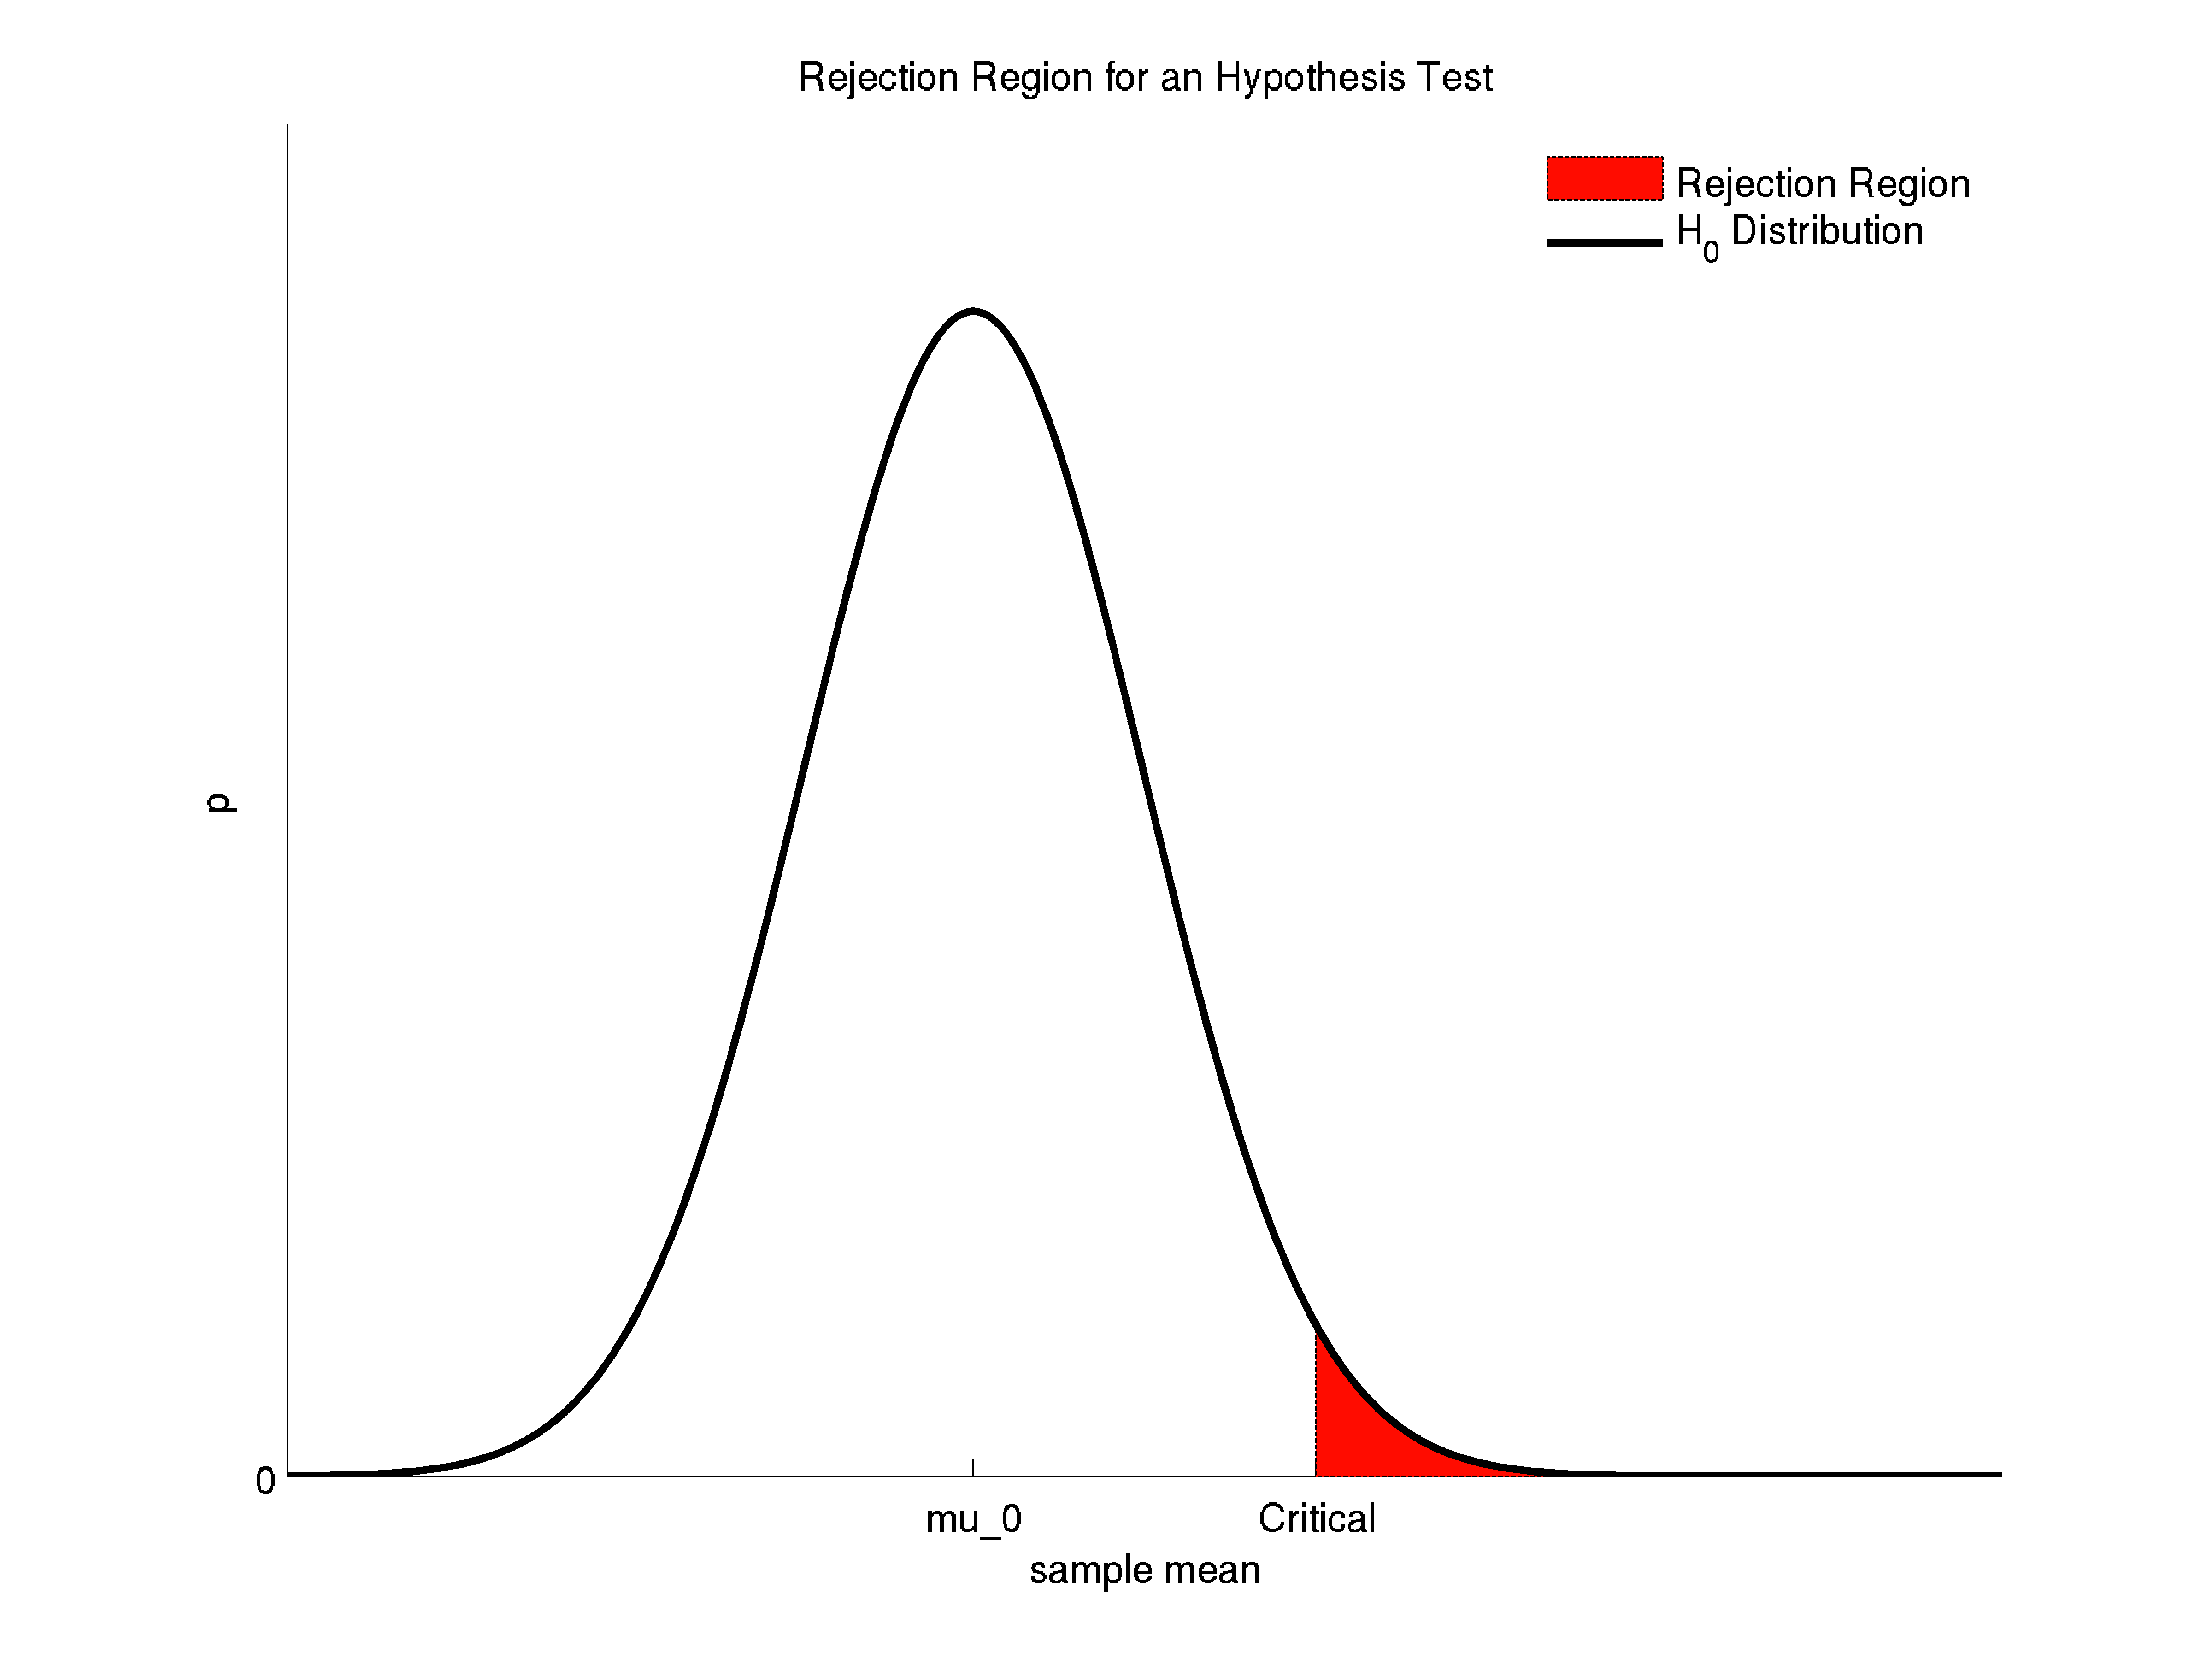
\includegraphics[width=6.0cm]{img/rejectionRegion}}
  }

  \only<2>{
    \centerline{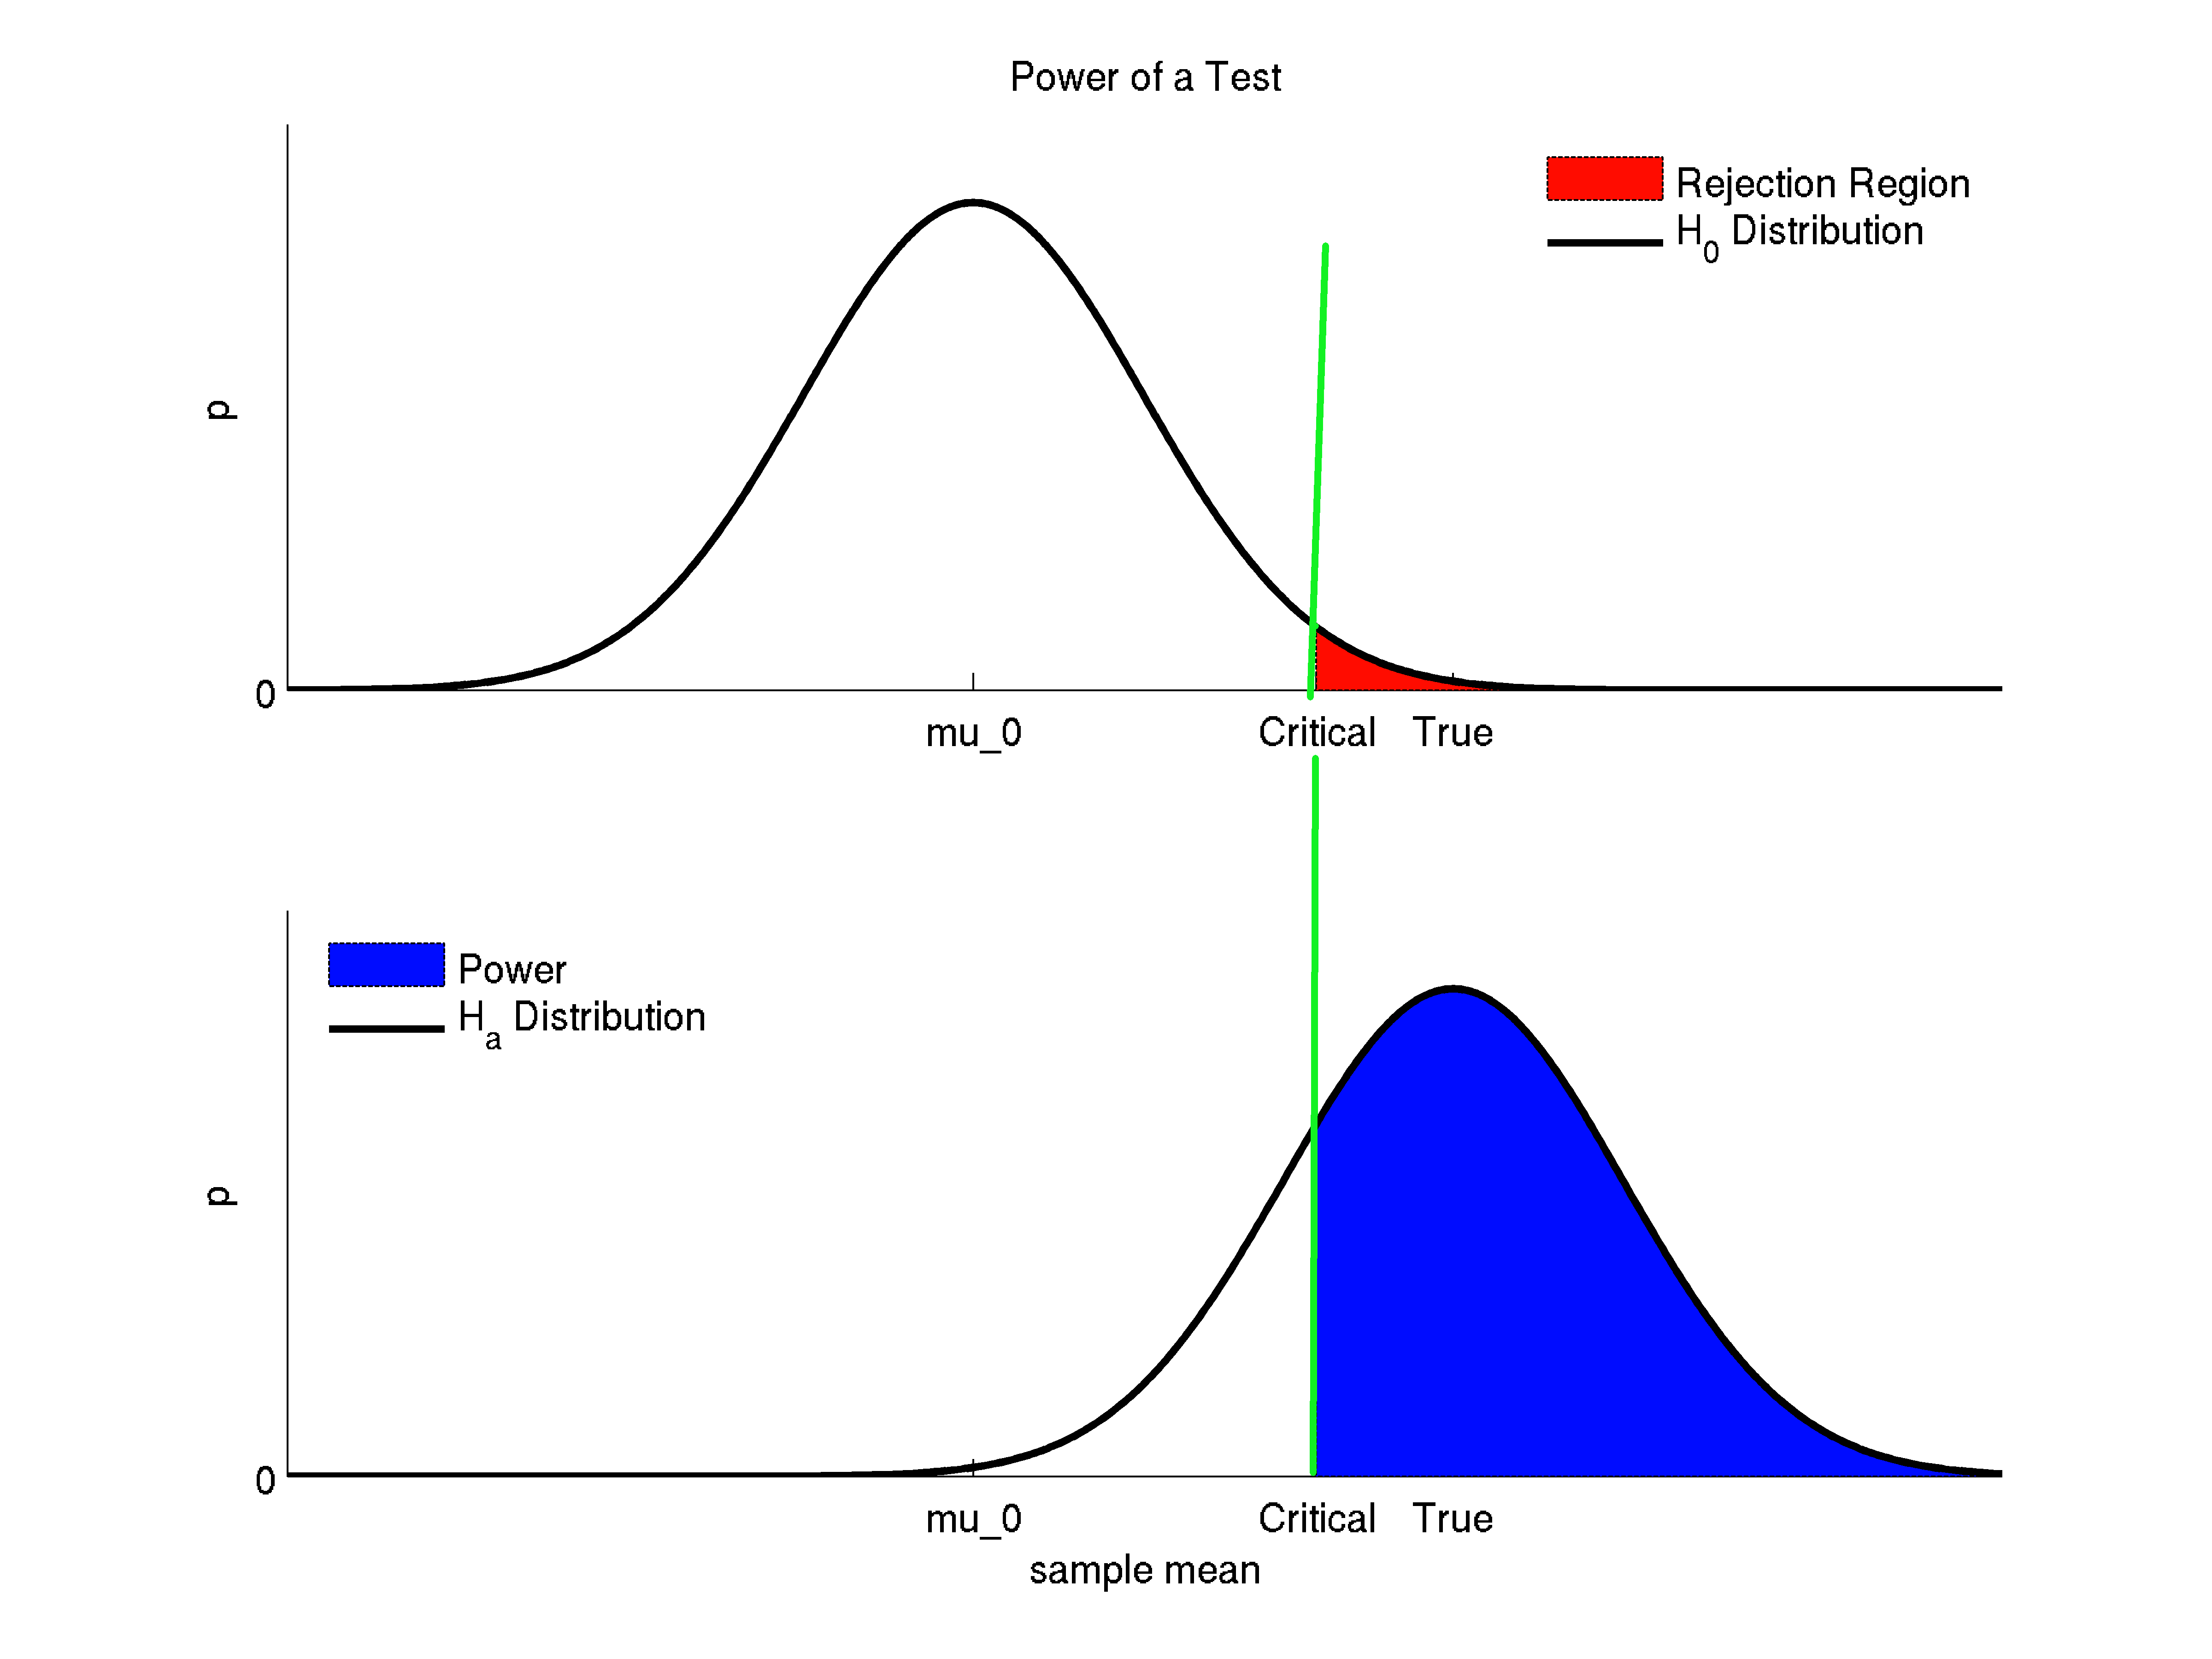
\includegraphics[width=6.0cm]{img/power}}
  }
  
\end{frame}


% LocalWords:  Clarkson pausesection hideallsubsections hideothersubsections
% LocalWords:  sectionstyle
